\chapter{Credit Mining System Design}
\label{chp:design}

% section overview, main components. Libtorrent as dependency. 
In this thesis, we introduce a ``Credit mining system'', an automatic investment framework that considers multiple properties of the swarms. With the credit mining system, a user can both gain credit and improve swarm performance with limited bandwidth allocation without any intervention necessary. We assume the \textit{credit} is the amount of bytes from the system to the community (and vice versa). From a higher perspective, credit mining system will help to keep a swarm alive by providing integral pieces to the peer who might need it. 

Firstly, the dependencies of the credit mining system, which is \textit{libtorrent}'s s\textit{hare mode}, will be elaborated. \texttt{Share mode} is a module which can be activated with the intent of helping a swarm, instead of normal content downloading. This module will be explained in detail in section \ref{section:sharemode}. After that, the design of the credit mining system is presented. This system consists of several subroutines which will be explained in section \ref{section:cmcomponents}. 

\section{Libtorrent's share mode}
\label{section:libtorrent}
\label{section:sharemode}
\bt~is simply a collection of specifications. It is free to be implemented in any language. One of most popular implementations is \textit{libtorrent}. \textit{Libtorrent} is written in \texttt{C++} and  has \texttt{python} binding. \textit{Libtorrent} was started in 2003 by Arvid Norberg, and it implemented most of the \bt~specifications. Most of the well-known extensions, such as DHT, PEX, magnet link, multi-tracker, and webseed have also been implemented. \textit{Libtorrent} is widely used by many torrent clients such as Deluge, qBittorrent, Free Download Managers, and many others.

One of the crucial features used in this work is \textit{share mode}\footnote{Core code of share mode can be found in \url{https://github.com/arvidn/libtorrent/blob/master/src/torrent.cpp\#L9586-L9727}}. Initial work performed by \citeauthor{2015:creditmining:capota} also used this feature \cite{2015:creditmining:capota}. Enabling share mode denotes that one is not interested in downloading the file in a swarm, but instead in gaining a higher share ratio. This is done by downloading as little as possible and uploading as much as possible. A swarm downloaded in share mode may never finish as \textit{libtorrent} will only download the pieces of a torrent which satisfy the share mode requirements.

The share mode algorithm works heuristically as it estimates the rarest piece available in the swarm based on the participating peers. The algorithm is presented in Algorithm \ref{alg:ltsharemode}. For clarity, we divide this algorithm in two parts. The first part is to pass all the restrictions. It tries to find missing pieces for each peer (line \ref{alg:l_lts:missingp}), disconnects some of the seeders because of connection limit (line \ref{alg:l_lts:disconnectpeers}), and reduces the number of missing pieces with twice the number of seeders (line \ref{alg:l_lts:reducemissing}). For the last, it is based on the assumption that seeders can upload as fast as the system. Share mode will fail if all missing pieces are expected to be provided by the seeders (line \ref{alg:l_lts:retmis}), upload ratio could not be reached (line \ref{alg:l_lts:retdlenough}), or too many parallel downloads (line \ref{alg:l_lts:retdling}).

The second part of share mode is to determine the rarest piece. \textit{Libtorrent} counts the number of peers for each piece to find the lowest one. The number of peers on the rarest piece is termed the \textit{rarity} of the piece. Share mode ensures that only the rarest piece available is downloaded (line \ref{alg:l_lts:rarepc}). The routine ends prematurely if there are not enough peers to upload the rarest piece (line \ref{alg:l_lts:rareunable}). Otherwise, it will randomly download the rarest pieces if there is more than one option (line \ref{alg:l_lts:dlrare}). 

\begin{algorithm}[h!]
	\caption{Libtorrent share mode algorithm}
	\label{alg:ltsharemode}
	\begin{algorithmic}[1]
		\Require{$T$ as share mode target}
		\Statex \hrulefill \Comment{Part 1}
		\State{$missing\_piece \gets 0$}
		\ForAll{$p \in connected\_peers$}
		\If{$p$ is a $leecher$ $and$ $p$ is not in share\_mode}	
		\State{$missing\_pieces$} += {$total\_pieces - pieces(p)$} \label{alg:l_lts:missingp}
		\EndIf	
		\EndFor
		\If{$|connected\_seeders|$ in $connected\_peer$ $>$ $90\%$}	
		\State disconnect excess seeder \label{alg:l_lts:disconnectpeers}
		\EndIf
		\State{$missing\_pieces$} -= {$2 \times |connected\_seeders|$}	\label{alg:l_lts:reducemissing}	
		\If{$missing\_pieces \leq 0$}  \label{alg:l_lts:retmis}
		\State \Return 
		\EndIf
		\If{$num\_downloaded \times T > uploaded$} \label{alg:l_lts:retdlenough}
		\State \Return
		\EndIf
		\If{$downloading > 5\% \times num\_downloaded$} \label{alg:l_lts:retdling}
		\State \Return
		\EndIf
		\Statex \hrulefill \Comment{Part 2}
		\State{$rarest\_rarity \gets MAX\_INTEGER$} 
		\ForAll{$pc \in pieces()$}
		\If{$pc$ not in $collected\_piece$ $and$ $peer\_count(pc) \leq rarest\_rarity$ }	\label{alg:l_lts:rarepc}
		\State{$rarest\_rarity \gets peer\_count(pc)$} 
		\State{$rare\_piece$.push($pc$)}
		\EndIf	
		\EndFor
		\If{$|connected\_peers| - rarest\_rarity < T$} \label{alg:l_lts:rareunable}
		\State \Return
		\EndIf
		\State download {$random(rare\_piece)$} \label{alg:l_lts:dlrare}
	\end{algorithmic}
\end{algorithm}

There are two limitations in this feature that we observed. Firstly, share mode did not check whether a swarm is good enough to perform this operation. It only tried to find popular pieces regardless of the swarm condition. Consequently, there is a possibility that the operation will not go well. For example, it is difficult to gain credit in a saturated swarm as there is not enough demand. Therefore, the user is fully responsible for whether share mode will yield high credit, or if it will waste his resource.

Secondly, the biggest limitation of share mode is the possibility of getting a bottleneck due to its strict policy. In the early stage of joining a swarm, share mode downloaded very few pieces at a time. For example, until the system has downloaded at least 20 pieces, it will only download one piece (5\%) at a time in share mode (line \ref{alg:l_lts:retdling}). It is also necessary to wait for that single piece to be uploaded (line \ref{alg:l_lts:retdlenough}) to at least $T$ peers. The combination of line \ref{alg:l_lts:retdlenough} and \ref{alg:l_lts:retdling} can result in slower decision making, by which time the rarity of pieces may have changed. If the system is too late to completely receive the piece, or the piece is not uploaded fast enough, this piece may be obsolete by that time as nobody wants it anymore. Therefore, the condition in line \ref{alg:l_lts:retdlenough} may never be satisfied. If the other pieces cannot cover this condition (by uploading to more than $T$ peers), then the operation will be unable to continue. Then, the system will neither download nor upload pieces anymore.

\section{Credit Mining Architecture}
\label{section:cmcomponents}

The credit mining system is intended to accomplish the assigned task automatically, with minimal user intervention. The way this system is designed is to align supply and demand of chosen swarm. The short term advantage of this approach is to gain credit by minimizing download and maximizing upload. In the long term, this potentially increases the overall performance of other users as well.

The system can be implemented on any torrent client. In Figure \ref{fig:cmcomponents}, it shows the compulsory elements and the relation between the \textit{credit mining system} and the \textit{torrent client}. Currently, we assume that every torrent client also tracks how much data a user has downloaded and uploaded in \textit{credit storage}. Naturally, any torrent client must have a so-called \textit{client downloader} module as well. \textit{Libtorrent} library also must exist as part of the dependencies. Another required feature is the ability to discover peers by all methods (DHT, PEX, LSD, and so on). In some cases, the peer discovery function is disabled for security reasons. While disabling any one method should not affect the credit mining system, it will reduce overall prospecting accuracy.

Credit mining system consists of several elements. Those are \textit{credit mining manager}, \textit{miners}, \textit{mining sources}, \textit{settings} object, and \textit{prospecting engine}. The \textit{manager} receives the \textit{settings} from user in the initial phase. To control the mining process, the user can only interact with the elements specified in \textit{settings}. User action is also limited to only adding and removing a \textit{mining source}. Each of the sources will be assigned with a \textit{miner}, and this assigning depends on the type of the source. The \textit{miner} also has sub-elements as part of the system. An in-depth explanation of mining source and \textit{miners} will be discussed in Section \ref{section:msource}. In the \textit{prospecting engine}, prospecting mechanism takes place. Prospecting mechanism as part of the investment methodology will be discussed in Chapter \ref{chapter:prospection}.

\begin{figure}[ht]
	\centering
 	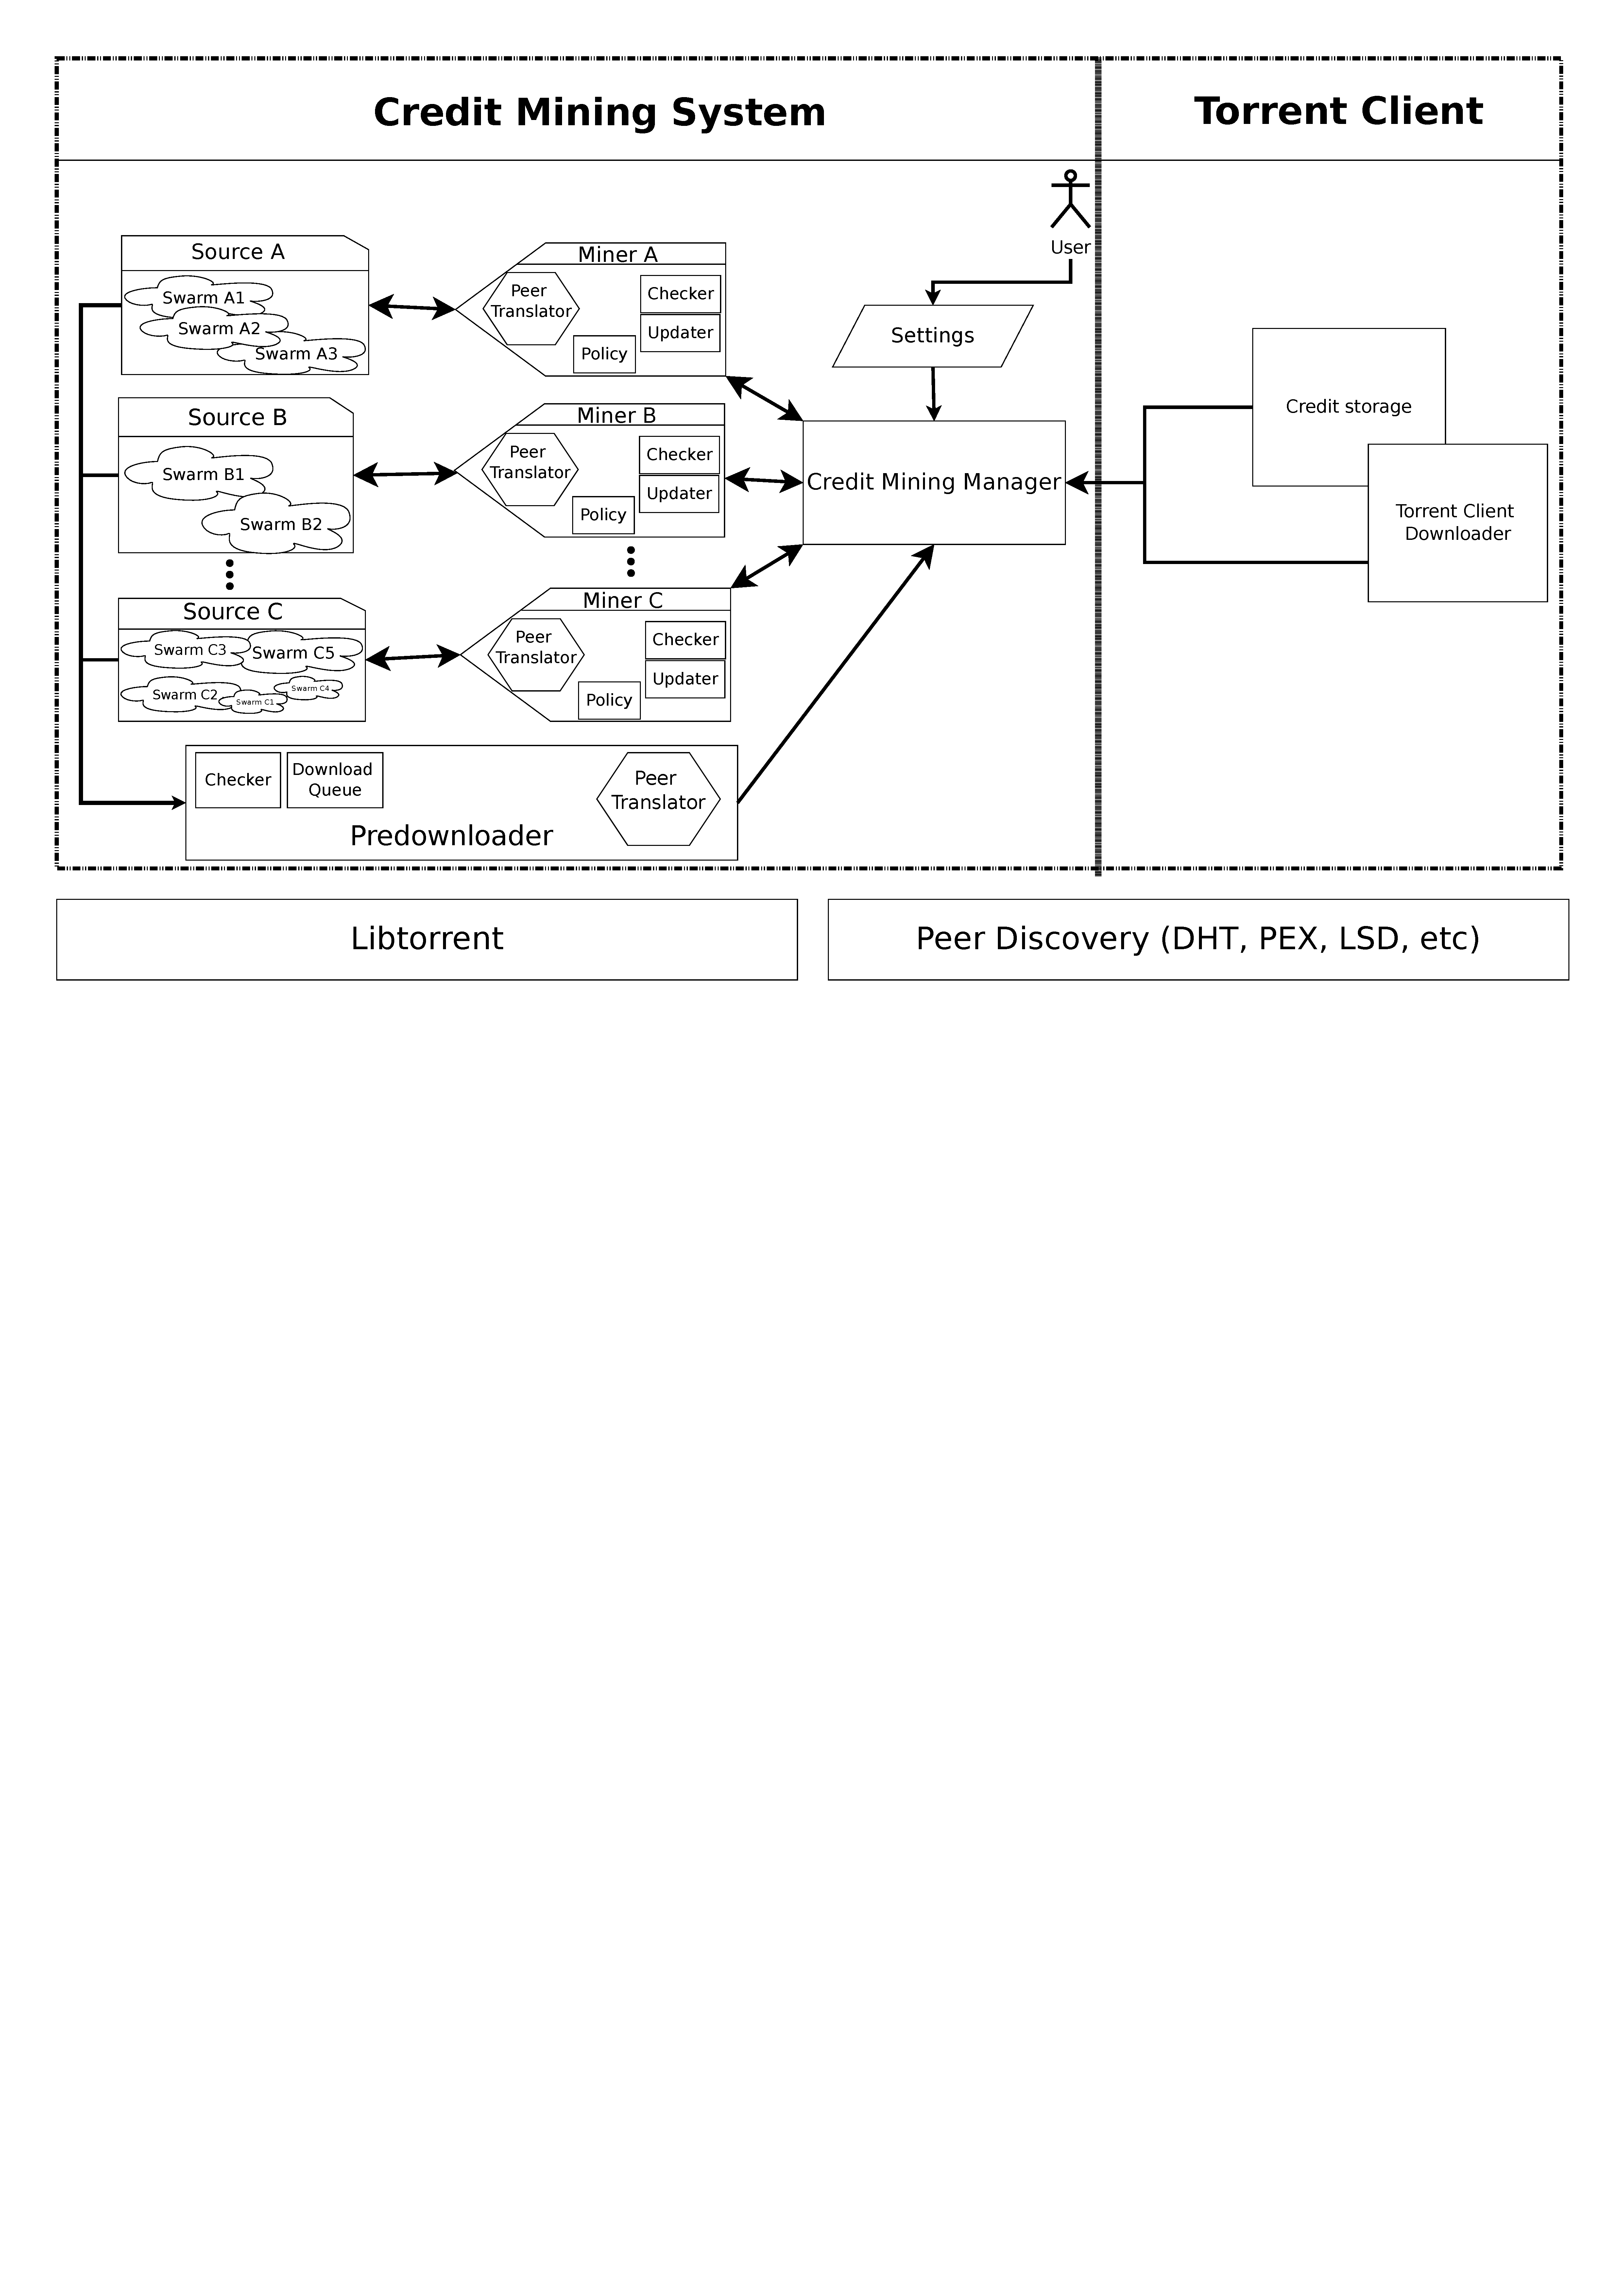
\includegraphics[width=\textwidth]{pics/cm_components.pdf}
	\caption{Credit mining components.}
	\label{fig:cmcomponents}
\end{figure}

% general flow
Before the credit mining system is executed, a user can change the settings used in the credit mining system. For example, if a user has a lot of memory available, it is desirable to mine many swarms at once by changing the \textit{max\_torrents\_active} parameter. Another example is if a user has a large amount of storage, decreasing \textit{share\_mode\_target} may yield in a better return. Some settings cannot be changed when the mining process is already running. Table \ref{tbl:cmsettings} shows the settings used in this system. 

After the user provides the setting and runs the \textit{credit manager}, the user can start mining by adding sources. A source usually consists of several swarms with different sizes, availability, and capacity. As mentioned previously, each of the sources will be assigned with one \textit{miner}. Before the miners start mining, the \textit{prospecting engine} fetches swarm information and then give the results to the manager .The manager will propagate the swarm information to miners and let the miners decide which swarm to mine based on that information. The manager also monitors the main torrent downloader to adjust the miners' bandwidth allocation. The credit gained from each of the miners will be reported to the manager, which then forwards the results to credit storage in the torrent client if necessary.

\begin{table}[h]
	\centering
	\caption{Credit mining settings}
	\label{tbl:cmsettings}
	\begin{adjustwidth}{-1.5cm}{}
	\begin{tabular}{|p{1cm}|p{4cm}|p{7cm}|p{2cm}|}
		\hline
		\rowcolor[HTML]{EFEFEF} 
		No. & Name & Description & Changeable at runtime \\ \hline
	1 & \textit{max\_torrents\_active} & The maximum number of simultaneous swarms that will be downloaded & Yes \\ \hline
	2 & \textit{max\_torrents\_per\_source} & The maximum number of stored torrents in a miner that will be considered for mining & Yes \\ \hline
	3 & \textit{source\_interval} & The interval needed to check for updates in the swarm & Yes \\ \hline
	4 & \textit{swarm\_interval} & The interval to re-evaluate the swarm and start/stop the swarm & Yes \\ \hline
	5 & \textit{share\_mode\_target} & Libtorrent share mode target (See Section \ref{section:sharemode}) & No \\ \hline
	6 & \textit{policy} & The policy used in mining (See Chapter \ref{chapter:prospection}) & No \\ \hline
	7 & \textit{tracker\_interval} & The interval to check for a new peer by peer discovery methods & No \\ \hline
	8 & \textit{timeout\_torrent\_activity} & The maximum time threshold to mark a swarm as 'inactive' & Yes \\ \hline
	9 & \textit{piece\_download} & The number of piece what will be downloaded in the \textit{prospecting} phase & No \\ \hline
	\end{tabular}
	\end{adjustwidth}
\end{table}



%The rest of this section will discuss key points of credit mining system. Several mining source types are supported with different treatment from miners. Prospecting methodology on top of libtorrent share mode will be elaborated afterwards. The methodology consists of two integral stages. Each of the stage has their own mechanism and requirements. Lastly, we will discuss other components that can support credit mining system of its prospecting, performance, and credit gain. 

\subsection{Mining Sources}
\label{section:msource} 
Currently, the credit mining system can accommodate three types of sources. These are: directory source, RSS source, and channel source. The miner will be initiated the moment the source is defined and added to the manager. A miner periodically monitors all of the swarms in the source.

The first type of source is called \textit{directory source}. The system takes and verifies the local directory path containing the \texttt{.torrent} file. Each of the files is examined and validated. Any corrupt or invalid file will be discarded and automatically deleted from the disk. The miner then sorts the files alphabetically and puts them into the queue. Both the directory and the queue are periodically monitored by the miner in case of the new incoming swarms. The miner will eventually pop an item from the queue one by one, build a suitable format for mining, and notify the manager to include this swarm.

The next possible mining source is from RSS (Rich Site Summary). RSS is a well-known method to fetch newly published data from the web. An RSS document contains the list of affected content which usually has summarized text and metadata. An RSS from a torrent portal such as etree\footnote{\url{http://bt.etree.org/rss/bt_etree_org.rdf}} and mininova\footnote{\url{http://www.mininova.org/rss.xml}} usually has the title, publication date and a link to the swarm. RSS also can easily be generated from private trackers for various purposes. We call the source of the RSS document as an \textit{RSS feed}. 

In \textit{RSS source}, we assume that the RSS link provided by the user is both available and valid. If by any case the retrieval of the content fails, the miner will stop immediately, notify the manager to disable the said source, and shut itself down. If the initial content retrieval is successful, the update mechanism will be launched periodically to fetch the newest content from the RSS feed. This content is then parsed, resulting in a list of swarm links and its associated information. The miner then asynchronously downloads the swarm metadata either via \texttt{.torrent} or magnet link. The same metadata will not be downloaded twice. After fetching the data, the miner will build a defined format for mining, and then notify the manager to include this swarm. 

\textit{Channel source} is the last type of source which is tightly related to the Tribler environment. As mentioned in section \ref{section:tribler} (Table \ref{tbl:community}), a channel is responsible for managing torrents and playlists in the Tribler community. A single channel can be discovered in the \textit{AllChannel} community. A channel is identified by a unique 40-length hexadecimal string. A Tribler user can create their own channel, put torrents into the channel, and share the channel with other users. When a user subscribes to a channel, they will be notified if a new torrent is added to that channel. Moreover, all torrents in the subscribed channel will be automatically downloaded into Tribler's database.

Given the identifier of a channel, the miner will continuously try to find and join the channel in \textit{AllChannel}. By joining the channel, the miner can get a list of torrents and its properties. After a miner joins the channel, the swarm metadata will be downloaded by a mechanism in Tribler. The miner then monitors the local database to determine whether new data has been fetched and whether there is a space for adding a new torrent to the manager. After knowing swarm information, the mining format will be built, and the manager will be notified of a ready swarm.

\subsection{User activity awareness}
\label{section:uactivityimpl}
Credit mining is an automatic system to download/upload to a swarm. If, at the same time, a user is downloading a swarm outside the one in the credit mining system, the bandwidth will be split. The user may experience a slower download speed and see this as a problem. We define \textit{user download activity} as an activity that is intentionally initiated by the user in order to participate in a particular swarm. Usually, this is the true purpose of having a torrent client. 

In response to that issue, we implemented another module in the credit mining system to adjust its mining activity to the user download activity. The credit mining system periodically observes whether there is user downloading activity. If there is none, then it can notify the miners to use all the bandwidth available. Otherwise, the system will limit the download and upload rate of mining activity to the remaining bandwidth available. At the period of observation, the mining download and upload rate will be set to zero.


\subsection{Resource Optimization}
\label{section:optimization}
In this section, we focus on several optimizations that can be implemented in the credit mining system. These optimizations are optional and can be omitted. However, as the system itself is not perfect, an improvement to support this system is advantageous. There are two optimizations in the credit mining system: duplicate elimination and swarm blacklisting.%, and reusing cache. 

In preliminary work by \citeauthor{2015:creditmining:capota}, credit mining system is able to distinguish duplicate content in P2P communities. It is highly possible that the same file might have a different \textit{infohash} as its identifier. The infohash of a swarm is an SHA1 hash consisting of 40-length hexadecimal string. An \textit{infohash} of a torrent can come from many factors such as different piece size, categorization as private or public swarm, or even the directory name of the files \cite{2015:creditmining:capota}. We used \textit{Levenshtein distance} to measure the difference between one swarm and another by considering the files in it, specifically its names and length. In the end, we only mine the swarms which have a higher number of seeders. Eliminating duplicate swarms can lead to the peer interaction being concentrated in one of the swarms. Thus, the performance of participating peer might be improved.

Despite all of the features in the credit mining system, there is no guarantee that it can constantly gain credit from a particular swarm. The bottleneck in share mode is one such example. We introduce \textit{swarm blacklisting} to remove and block low-performance swarms. The miner periodically watches whether data are constantly being downloaded or uploaded from a particular swarm. If no activity is detected from that swarm for a long period of time, the miner will remove the swarm from its library and block it. That means this particular swarm cannot be chosen by any of the swarm selection policies. It will be added to the library again only after several rounds. If, by any chance, the library is empty and there are swarms blacklisted, those will be added to the library again.

%In the prior work, it is important to note that after mining for a certain swarm was stopped, miners will delete downloaded files to save the storage. Although it is safe for the system to discard downloaded files, the resource used to redownload piece will be costly. This issue is fixed in current credit mining system. Files from a swarm that has been stopped for mining is archived with its history and stored in \textit{cache}. The history consists of the index of the piece that have been downloaded, peer information, statistics, and many others. When mining restarts, if there are new peers requesting piece the system already have, it can be immediately uploaded without need to redownload or check the piece.